\newpage
\subsubsection{Phasenverschiebung}

\hfill \break
\begin{itemize}
    \item allgemein: $y=sin(deg(x+c))$
    \item wen $c > 0 \rightarrow$ verschiebung Links
    \item wen $c < 0 \rightarrow$ verschiebung Rechts
\end{itemize}

\hfill \break
\begin{itemize}
    \item Grund-Sin Funktion $\rightarrow$ \textcolor{red}{$sin(deg(x))$}
    \item Rechtsverschiebung $\rightarrow$ \textcolor{green}{$sin(deg(x - \frac{\pi}{2}))$}
    \item Linksverschiebung $\rightarrow$ \textcolor{blue}{$sin(deg(x + \frac{\pi}{2}))$}
\end{itemize}


\hfill \break
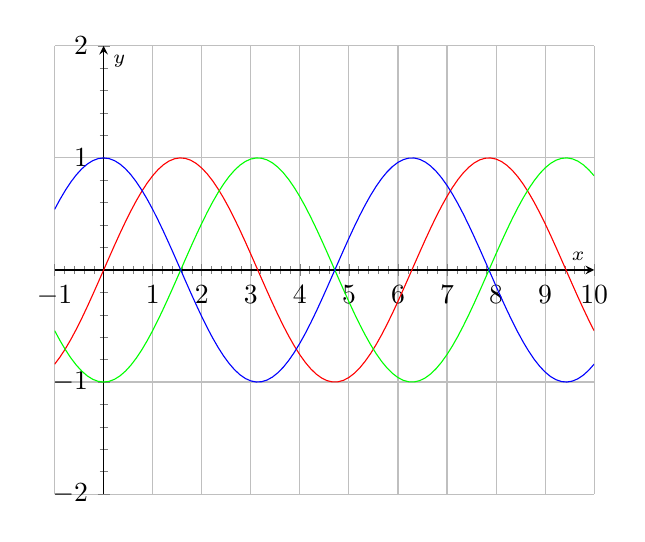
\begin{tikzpicture}[scale=1]
    \begin{axis}%
        [
            grid=major,
            xtick={-1,0,...,10},
            minor x tick num=4,
            xmin=-1,
            xmax=10,
            xlabel={\scriptsize $x$},
            axis x line=middle,
            ytick={-2,-4,...,2},
            minor y tick num=4,
            ymin=-2,
            ymax=2,
            ylabel={\scriptsize $y$},
            axis y line=middle,
            no markers,
            samples=100,
            domain=-1:10,
        ]
        \addplot[red] (x,{sin(deg(x))});
        \addplot[green] (x,{sin(deg(x - (pi / 2)))});
        \addplot[blue] (x,{sin(deg(x + (pi / 2))))});
    \end{axis}
\end{tikzpicture}